\section{Numerical Methods}

In this section, we aim to find a numerical approximation $\{x_n\}$ to $x(t)$ at discrete times $t_n$.

In general, we take a differential equation of the form
\[
x' = f(x, t),
\]
and times $t_n$ are given by
\[
t_n = t_0 + nh,
\]
where $h$ is the time step.

\subsection{Euler's Method}

The Euler Method involves approximating $x_{n+1}$ using the tangent line (see \Cref{fig:euler}). To see this, observe that
\[
\frac{x(t_{n+1}) - x(t_n)}{t_{n+1} - t_n} = \frac{x(t_{n+1}) - x(t_n)}{h} \approx f(x(t_n), t_n).
\]
Replacing the exact values $x(t_n)$ with $x_n$ and rearranging, we find the following iterative formula that is Euler's Method:
\begin{equation}\label{eq:euler}
	x_{n+1} = x_n + h f(x_n, t_n).
\end{equation}

\begin{figure}[!ht]
	\centering
	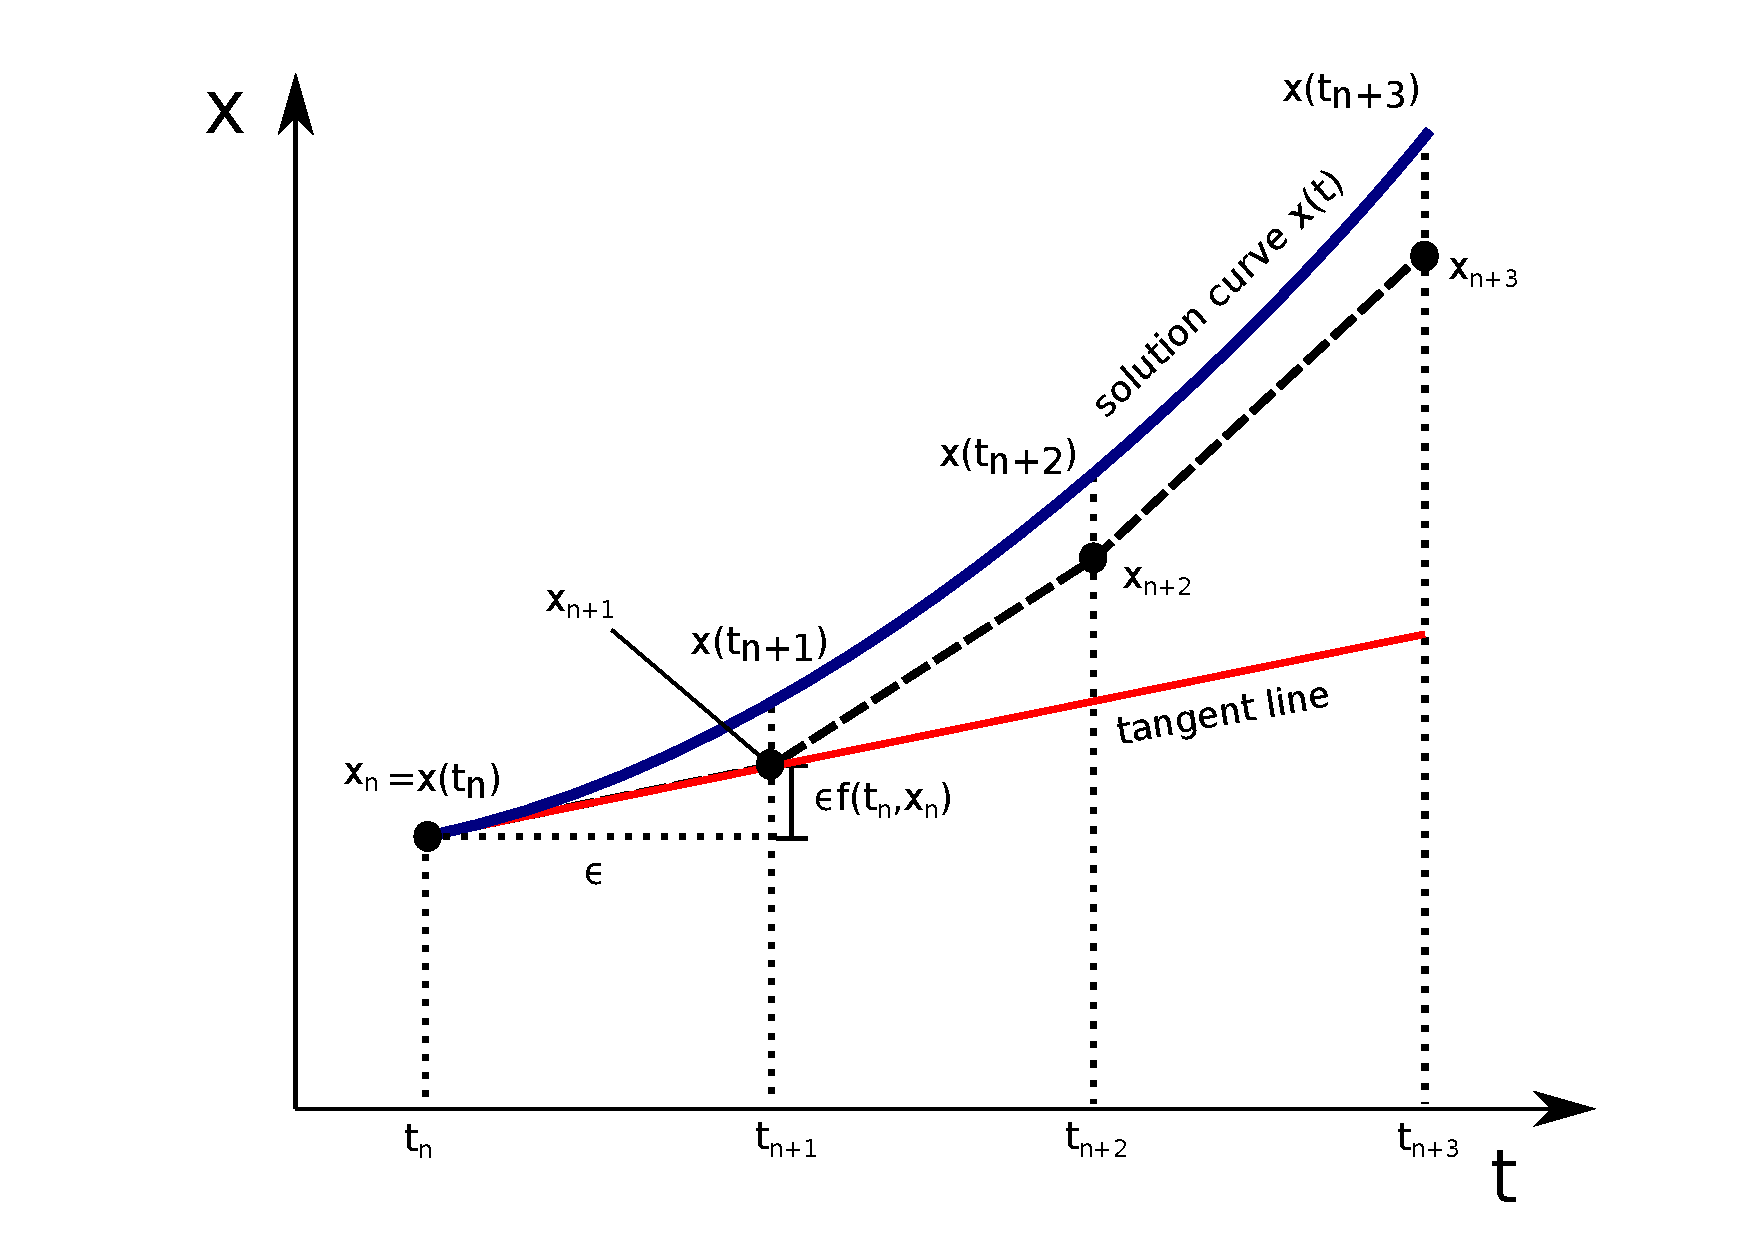
\includegraphics[width=0.65\textwidth]{euler.pdf}
	\caption{Illustration of multiple iterations of Euler's method. Note that $\epsilon$ in this diagram is equivalent to our time step $h$. \cite[Figure 2]{numgraph}.}
	\label{fig:euler}
\end{figure}

There are a couple of general ways of deriving numerical approximations:
\begin{enumerate}
	\item{\textbf{Integral Equation:} \[x(t_{n+1}) = x(t_n) + \int_{t_n}^{t_{n+1}} f(x(s), s) \,ds.\] Then different approximations arise by considering ways that $\int_{t_n}^{t_{n+1}} f(x(s), s) \,ds$ may be approximated though the area under the curve.}
	\item{\textbf{Taylor Expansion:} \[x(t_{n+1}) = x(t_n + h) = x(t_n) + hx'(t_n) + \frac{h^2}{2}x''(t_n) + \cdots\] From this, approximations may be made by, for example, taking the first $k$ terms of the expansion. Another useful form of Taylor's theorem is the following: \[x(t_n + h) = x(t_n) + hx'(t_n) + \frac{h^2}{2}x''(\overline{t}_n)\] for some $\overline{t}_n$ between $t_n$ and $t_{n+1}=t_n+h$.}
\end{enumerate}

\begin{exercise}
	Derive \Cref{eq:euler} using both the method of integral equations (see \Cref{fig:eulerint}) and using the Taylor expansion.
\end{exercise}

\begin{figure}[!ht]
	\centering
	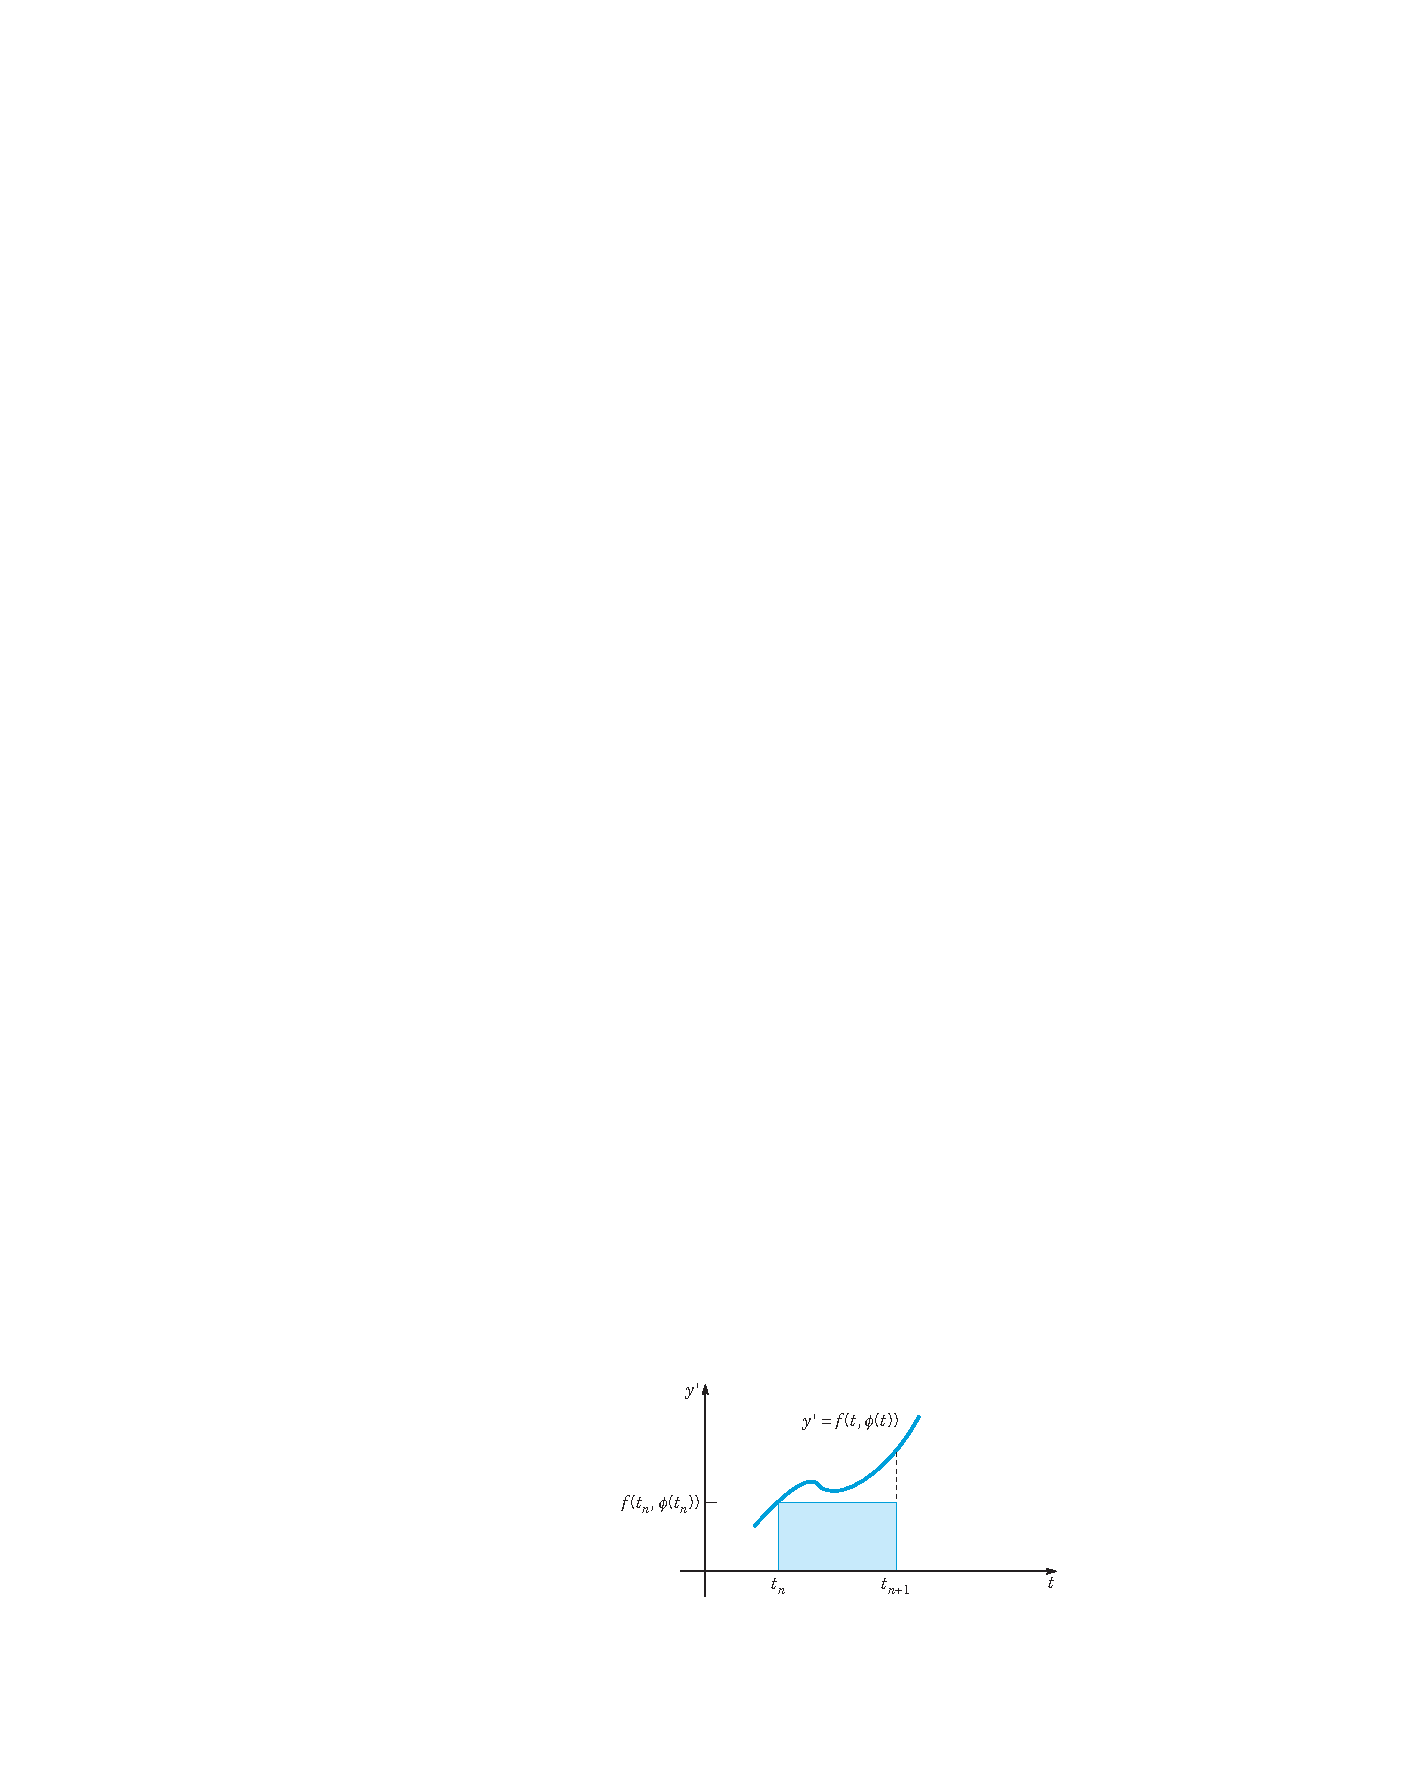
\includegraphics[width=0.6\textwidth]{integralEquationEuler.pdf}
	\caption{Derivation of the Euler method using the integral equation \cite[Figure 8.1.1]{boyce}.}
	\label{fig:eulerint}
\end{figure}

The formula in \Cref{eq:euler} is also called the Forward Euler Method, and its cousin is the Backward Euler Method. We can derive this method using the integral equation and approximating the integral by a rectangle with width $h$ and height $f(x_{n+1}, t_{n+1})$:
\begin{equation}
	x_{n+1} = x_n + h f(x_{n+1}, t_{n+1}).
\end{equation}

Note that this is an implicit method (requiring extra work to solve for $x_{n+1}$) compared to the Forward Euler which is explicit.

Once we are comfortable with representing the differential equation as an integral equation and approximating areas, we can find many more schemes for numerical approximations, for example the Trapezoidal rule (illustrated in the case where $f$ does not depend on $t$):
\begin{equation}
	x_{n+1} = x_n + h \frac{f(x_n)+f(x_{n+1})}{2}.
\end{equation}
and the Implicit Midpoint rule:
\begin{equation}
	x_{n+1} = x_n + h f\left(\frac{x_n+x_{n+1}}{2}\right).
\end{equation}

\subsection{Errors}

In a numerical approximation, there are three sources of errors:
\begin{enumerate}
	\item Approximation of $x' = f(x,t)$ between $x_n$ and $x_{n+1}$.
	\item Error in $x_n$ (because of errors incurred in previous steps).
	\item Round off errors.
\end{enumerate}

We will consider three types of errors:
\begin{enumerate}
	\item Global truncation error: $E_n = x(t_n) - x_n$.
	\item Round off error: $R_n = x_n - X_n$, where $X_n$ is the result with round-off.
	\item Local error $e_n = x(t_n) - x_n^*$, where $x_n^*$ is the error incurred after one time step by assuming we start on the true curve.
\end{enumerate}

In practice, it may be required to take the absolute value of $E_n$, $R_n$, and $e_n$ since we want the error measurement to be positive.

\begin{eg}
	We will calculate the local and global errors in the Forward Euler Method. Beginning with the Taylor expansion:
	\begin{align*}
		x(t_n) &= x(t_{n-1} + h) \\ 
		&= x(t_{n-1}) + hx'(t_{n-1}) + \frac{h^2}{2}x''(\overline{t}_n) \tag{$t_{n-1} \leq \overline{t}_n \leq t_n$} \\
		&= x^* + hf(x^*, t_{n-1}) + \frac{h^2}{2}x''(\overline{t}_n).
	\end{align*}
	In addition,
	\[
	x_n = x^* + h f(x^*, t_{n-1}),
	\]
	therefore
	\[
	x(t_n) - x_n = e_n = \frac{h^2}{2}x''(\overline{t}_n).
	\]
	If $x''(t)$ is bounded, then we can write
	\[
	|e_n| \leq M h^2 \implies e_n = O(h^2).
	\]
	Now to find the global error by supposing that we make the local error $n$ times:
	\begin{align*}
		E_n &= x(t_n) - x_n, \quad n = \frac{t_n-t_0}{h} \\
		|E_n| &\leq M h^2 n = M h^2 \frac{t_n-t_0}{h} = Kh \\
		\implies E_n &= O(h).
	\end{align*}
	Therefore we say that the Forward Euler Method is a first-order method (or that it is first-order accurate).
\end{eg}

\begin{remark}
	Generally, a method is of order $p$ if $|E_n| \leq K h^p$ i.e. $E_n = O(h^p)$.
\end{remark}

\subsection{Heun Method}

To derive the Heun Method, we begin with the integral equation
\begin{align*}
	x(t_{n+1}) &= x(t_n) + \int_{t_n}^{t_{n+1}} f(x(s), s) \,ds \\
	&\approx x(t_n) + \frac{h}{2} (f(x(t_n), t_n) + f(x(t_{n+1}), t_{n+1})),
\end{align*}
using a trapezoidal approximation of the integral (see \Cref{fig:heunint}).

Now, we can use the approximation
\[
x(t_{n+1}) \approx x(t_n) + h f(x(t_n), t_n)
\]
(i.e. the Forward Euler Method) to write
\begin{equation}
	x_{n+1} = x_n + \frac{h}{2}\left[f(x_n,t_n) + f(x_n + hf(x_n,t_n), t_{n+1})\right].
\end{equation}
This is the Heun Method (or Heun's Method).

\begin{figure}[!ht]
	\centering
	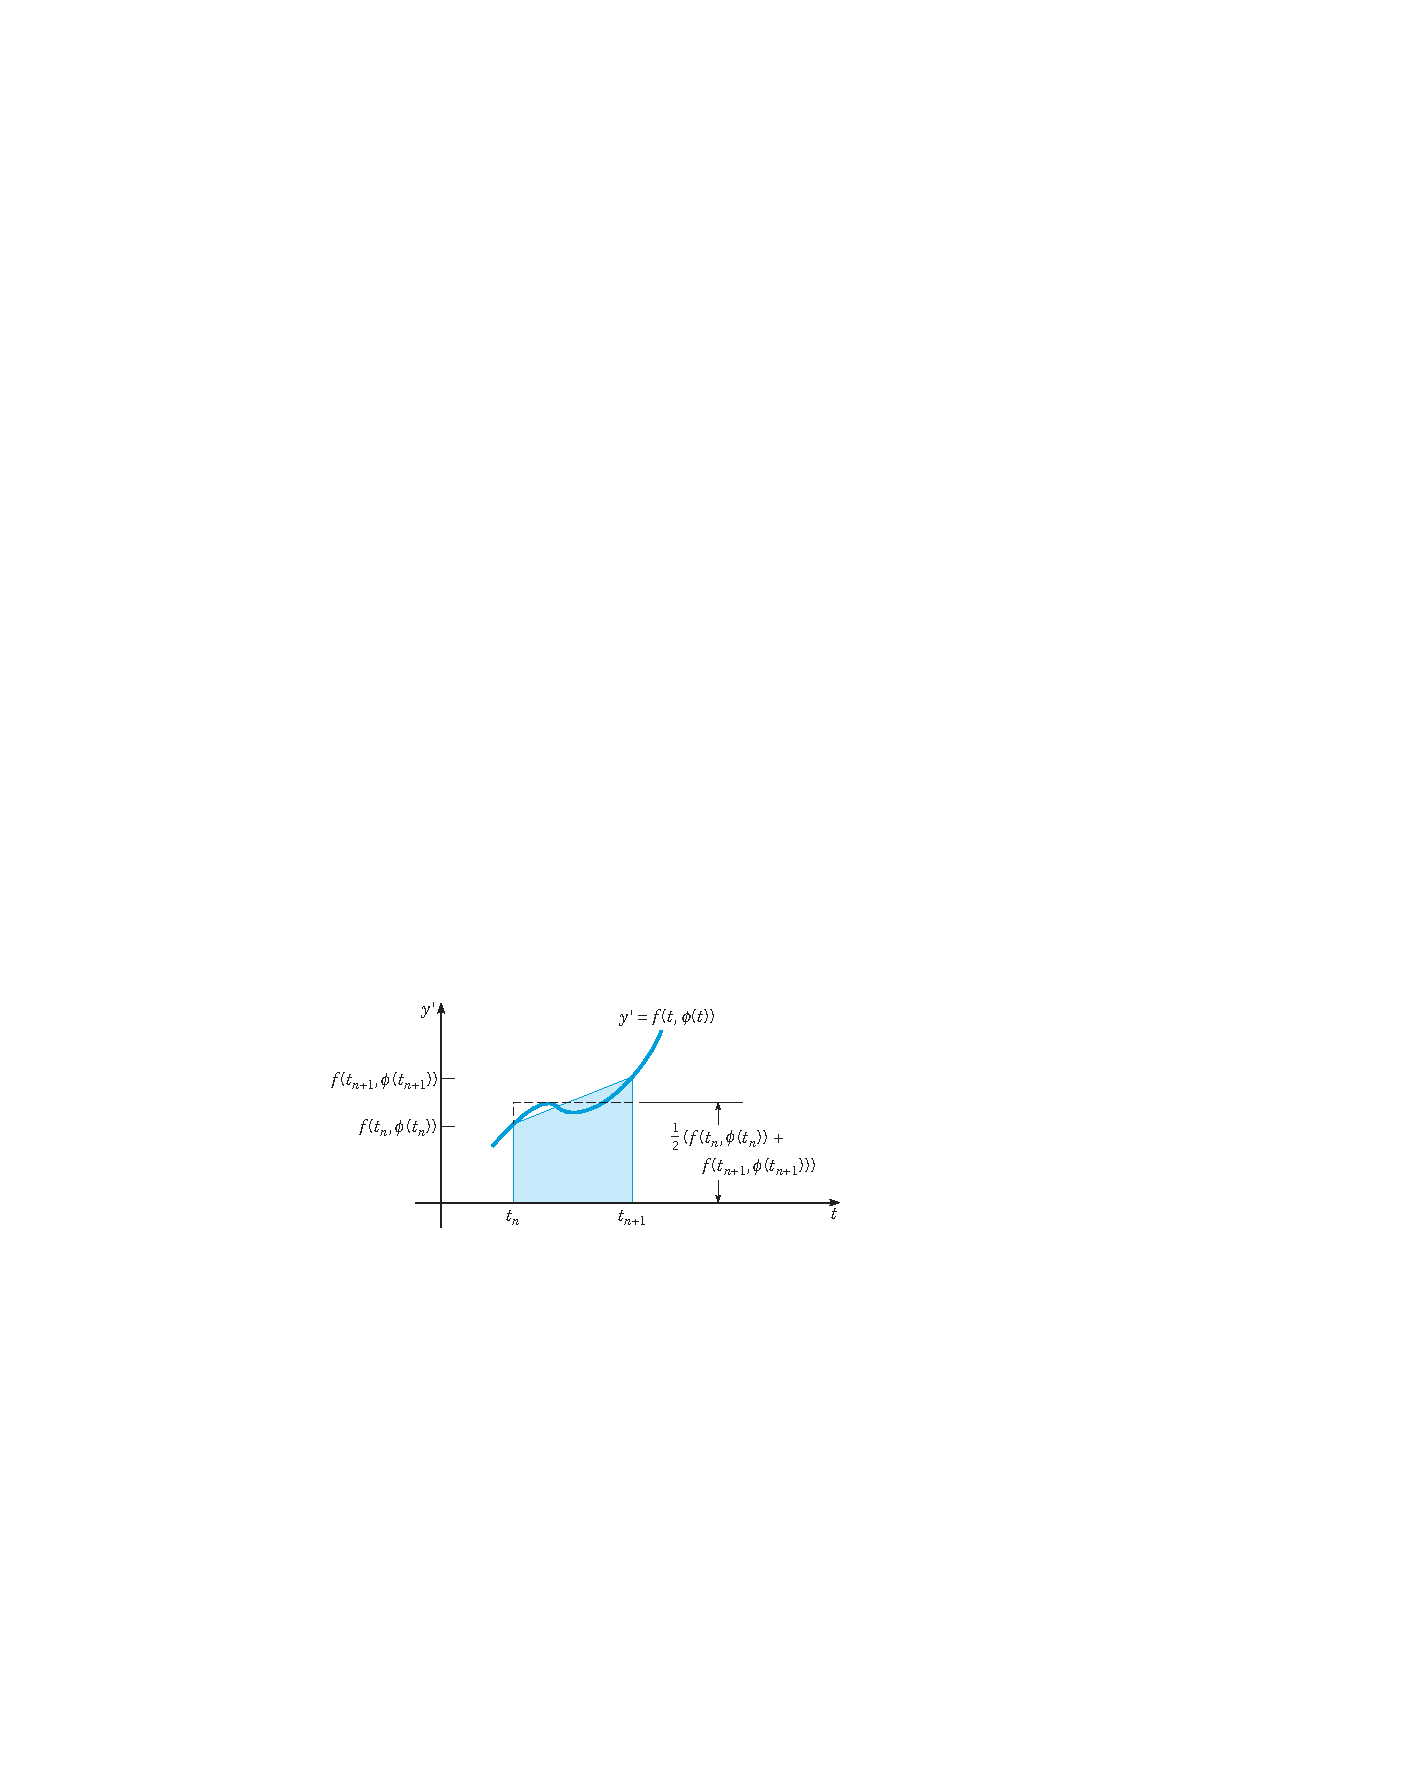
\includegraphics[width=0.6\textwidth]{integralEquationHeun.pdf}
	\caption{Derivation of the Heun method using the integral equation \cite[Figure 8.2.1]{boyce}.}
	\label{fig:heunint}
\end{figure}

\begin{remark}
	It can be shown that the local error of this method if $O(h^3)$ and the global error is $O(h^2)$, this the order of Heun's Method is 2.
\end{remark}

Heun's Method is an example of a multistage method. Compared to a single-step method like Euler's Method where only one point and its derivative was used to determine the next value, a multistage method takes some intermediate steps and then refers to multiple previous points in the final calculation. To see this explicitly, we can express Heun's Method as follows, with two explicit 'steps' $k_1$ and $k_2$:
\begin{align*}
	k_1 &= f(x_n, t_n) \\
	k_2 &= f(x_n + hk_1, t_n+h) \\
	x_{n+1} &= x_n + \frac{h}{2}(k_1 + k_2).
\end{align*}

\subsection{Runge-Kutta Methods}

A family of multistep methods is the group of Runge-Kutta methods. The most widely known member of this family is the four-step version (also known as RK4), which may be illustrated as follows:
\begin{align*}
	k_1 &= f(x_n, t_n) \\
	k_2 &= f(x_n + \frac{hk_1}{2}, t_n + \frac{h}{2}) \\
	k_3 &= f(x_n + \frac{hk_2}{2}, t_n + \frac{h}{2}) \\
	k_4 &= f(x_n + hk_3, t_n + h) \\
	x_{n+1} &= x_n + \frac{h}{6} (k_1 + 2k_2 + 2k_3 + k_4).
\end{align*}

This is a fourth order method, i.e. $E_n = O(h^4)$ and $e_n = O(h^5)$.

\subsection{Adams-Bashforth Method}

This family of methods uses $x_n, x_{n-1}, \dots$ to compute $x_n$. We take the case of using only $x_n$ and $x_{n-1}$. 

Reminding ourselves of the integral equation,
\[
x(t_{n+1}) = x(t_n) + \int_{t_n}^{t_{n+1}} f(x(s), s) \,ds,
\]
we approximate $f$ by $f(s) = as + b$.\footnote{Note that this illustration is for an autonomous system, i.e. one where $f$ does not depend on $t$, but an analogous form of the method exists for non-autonomous systems.}

We then must find $a$ and $b$ such that 
\begin{align*}
	f(x_{n-1}) &= a t_{n-1}+b \\
	f(x_n) &= a t_n + b.
\end{align*}

Solving for $a$ and $b$, we obtain
\[
a = \frac{f(x_n)-f(x_{n-1})}{h} \quad \text{and} \quad b = \frac{f(x_{n-1})t_n - f(x_n)t_{n-1}}{h}.
\]

Returning to the integral equation,
\[
x_{n+1} = x_n + \int_{t_n}^{t_{n+1}} as + b \,ds = a \frac{t_{n+1}^2 - t_n^2}{2} + b(t_{n+1} - t_n).
\]

To simplify, we first write $t_{n+1}^2 - t_n^2 = (t_{n+1} - t_n)(t_{n+1}+t_n) = h (t_{n+1}+t_n)$ for constant step size $h = t_{n+1} - t_n$. Then
\begin{align*}
	\frac{a}{2}(t_{n+1}^2 - t_n^2) + b(t_{n+1} - t_n) &= \frac{f_n - f_{n-1}}{2}(t_{n+1}+t_n) + f_{n-1}t_n - f_n t_{n-1} \\ 
	&= \frac12(f_n t_{n+1} + f_nt_n - f_{n-1}t_{n+1} - f_{n-1}t_n) + f_{n-1}t_n - f_n t_{n-1} \\ 
	&= f_n(\frac12 t_{n+1} + \frac12 t_n - t_{n-1}) + \frac12 f_{n-1}(t_n - t_{n+1}).
\end{align*}

Then $t_n - t_{n+1} = -h$ clearly, and $\frac12 t_{n+1} + \frac12 t_n - t_{n-1} = \frac12 t_n + \frac12 h + \frac12 t_n - t_{n-1} = \frac32 h$, hence we get the following simplified formula:
\begin{equation}
	x_{n+1} = x_n + \frac{h}{2}\left(3f(x_n) - f(x_{n-1})\right).
\end{equation}

\vfill
\pagebreak
\subsection{Comparison of Methods in Practice}

A comparison of the four methods discussed in this section is shown in \Cref{fig:numericals}. The particular example is the harmonic oscillator, where
\begin{align*}
	x' &= y \\
	y' &= -x.
\end{align*}

\begin{figure}[!ht]
	\centering
	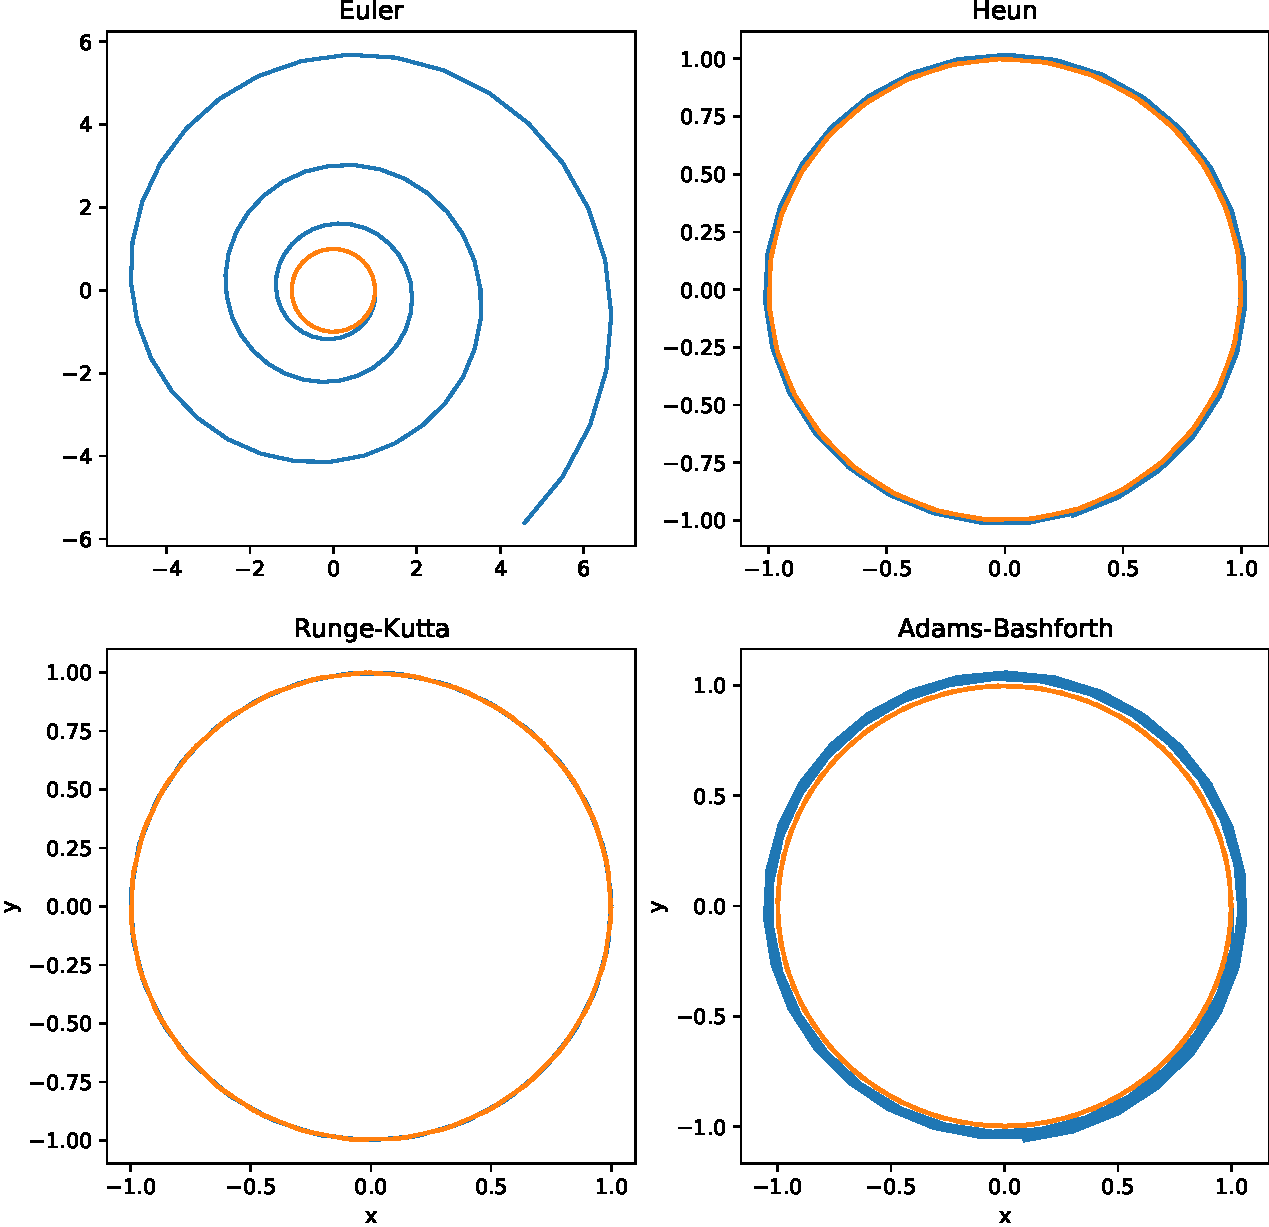
\includegraphics[width=0.9\textwidth]{NumericalMethods.pdf}
	\caption{Comparison of the results of the Euler, Heun, Runge-Kutta, and Adams-Bashforth methods (blue) in approximating an ODE. The true solution is shown in orange.}
	\label{fig:numericals}
\end{figure}